\documentclass[english,fleqn,allpages]{ISTE_science}[2018/07/30]


\setcounter{MaxMatrixCols}{30}
\usepackage{amsthm}
%\usepackage{OKS_ISTE}
%\CropMarksOn
\usepackage{natbib}
\renewcommand\bibsection{\section{\bibname}}
\setlength{\bibsep}{3pt} 
\makeatletter

%\newcounter{numdef}[chapter] \global\long\def\thenumdef{\thechapter.\arabic{numdef}}
% \global\long\def\NumberedDefinition#1


\newsavebox{\fminibox} \newlength{\fminilength} \newenvironment{fminipage}[1][\linewidth]{%
 \setlength{\fminilength}{#1 - 2\fboxsep - 2\fboxrule}
 \begin{lrbox}{\fminibox}
  \begin{minipage}{\fminilength}}{%
  \end{minipage}
 \end{lrbox}
 \noindent
 \fbox{\usebox{\fminibox}}}


\title{Hierarchy and co-evolution processes}
%
%\maketitle
%Rheology of non-spherical particle suspensions]%{%
%Setting Monographs and Edited Collections\\
%According to the \hermes{} Guidelines\\
%with the \oh{} Package}


%\author{%
%Roger \Name{Rousseau} (class, styles, and tools design)\\[2pt]
%Christian \Name{Scheen} (English documentation)}


%\date{%
%Version~\PackageVersion{}, \filedate{}}


\begin{document}
\raggedbottom
%\hbadness=2000 \emergencystretch=2em \lefthyphenmin=3 \righthyphenmin=3

%\frontmatter

%\maketitle
%\tableofcontents

%\raggedbottom
\mainmatter
%\setcounter{chapter}{9}
\chapter{Hierarchy and co-evolution processes}%{Juste \Name{Raimbault}}
\label{chap-struct}

\markboth{Hierarchy and co-evolution processes}{Hierarchy and co-evolution processes}


\authorname{Juste \Name{Raimbault}}{Center for Advanced Spatial Analysis, University College London}


% book subject "Centralités et hiérarchies des réseaux et des territoires"
% => specific geo of networks and territories


%%%%%%%%%%%%%%%%
\section{Introduction}


\subsection{Complexity and hierarchy}

Complex systems with emergent properties through self-organization processes are also most of the time exhibiting some kind of hierarchical structure. Although the term of hierarchy has several different definitions and uses in very different disciplines, ranging from political science \citep{crumley1987dialectical} to physics \citep{10.1371/journal.pone.0033799}, it seems to be intrinsically linked with complexity. \cite{lane2006hierarchy} classifies four frequent uses of the term hierarchy, namely (i) order hierarchy corresponding to the existence of an order relation for a set of elements, (ii) inclusion hierarchy which is a recursive inclusion of elements within each other, (iii) control hierarchy which is the ``common sense'' use of the term as ranked entities controlling other entities with lower rank, and (iv) level hierarchy which captures the multi-scale nature of complex systems as ontologically distinct levels (or scales). For the particular study of social systems, he concludes that hierarchical levels may be entangled, that upward and downward causations are both essential, and that at least three levels (micro, meso, macro) are generally needed to capture the complexity of such systems. In a more philosophical account of complexity, \cite{morin1980methode} constructs a hierarchical method of interdisciplinary knowledge, insists on the tension between dependancy and interdependency or between opening and closing (rejoining ideas from \cite{holland2012signals}), and develops an implicit hierarchy of social systems when hypothesizing the emergence of third-type societies (swarm intelligence between humans).

Different types of complexity may be related to different types of hierarchy as \cite{raimbault:halshs-02089520} proposes, and hierarchy would indeed be endogenous to theories of complexity. \cite{allen2017multiscale} develop a multiscale information theory in which the information profile across scales, or hierarchical levels, allows quantifying the complexity of a system. The complex adaptive system theory of \cite{holland2012signals} considers complex systems as systems of boundaries that filter signals, implying an inclusion and scale hierarchy between boundaries. Theories of scaling as the one synthesized by \cite{west2017scale} rely on the quantification of hierarchy in certain dimensions of systems, captured by exponents of scaling laws. Hierarchy may be endogenous to complexity, or to knowledge of the complex itself, since for example \cite{fanelli2013bibliometric} provides empirical evidence of a ``hierarchy of sciences'', in the sense of possibility to reach theoretical and methodological consensus. This corresponds in some sense to the ``ontological complexity'' of \cite{pumain2003approche}, which relies on the number of viewpoints needed to grasp a system, or the number of perspectives in an applied perspectivism framework \citep{2018arXiv181104270R}. Wether linked to systems themselves or to models and theories of them, hierarchy appears to be tightly linked to complexity.



\subsection{Territorial systems and hierarchy}


Urban systems, and more generally territorial systems, are particularly linked to hierarchy \citep{pumain2006hierarchy}: they indeed encompass all the meanings aforementioned (order hierarchy between settlement sizes for example, inclusion hierarchy between territorial boundaries, control hierarchy through governance structure, and more importantly level hierarchy through their multi-scalar nature). \cite{batty2006hierarchy} shows that hierarchies are inherent to urban systems, as fat tail distribution of settlement size are already produced by simple models of urban growth, and suggests also that urban design processes imply underlying overlapping hierarchies. \cite{pumain2006alternative} links hierarchical selection and hierarchical diffusion of innovation across cities to the long-term dynamics of urban systems. \cite{pumain:halshs-02303136} recalls that interactions in systems of cities are tightly linked to the emergence of urban hierarchies. Generally, scaling laws in urban systems can be considered as systematic manifestations of a hierarchical structure \citep{pumain2004scaling}, which is more complex than a simple order hierarchy, since scaling patterns vary with the definition of cities \cite{cottineau2017diverse}

Several dimensions of urban systems exhibit hierarchical properties, as transportation networks and transportation flows \citep{jiang2009street}, the global distribution of multinational firms \citep{godfrey1999ranking}, or governance structures \citep{li2015administrative}.





\subsection{Co-evolution and hierarchy}



Hierarchy in complex systems is furthermore intrinsically linked to the concept of co-evolution. Following \cite{lane2006hierarchy}, the approach to complex adaptive systems proposed by \cite{holland2012signals} integrates levels and nested hierarchies, since it considers complex systems as ensembles of boundaries that filter signals. 

In the context of economic geography and the co-evolution of firms, \cite{volberda2003co} distinguishes between a genealogical hierarchy (evolutionary processes in the biological sense) and an ecological hierarchy (co-evolutionary economic processes). % TODO check this



\subsection{Proposed approach}

\cite{pumain2006introduction} recalls in the context of social systems some remaining methodological questions: how are hierarchies produced? How do hierarchies evolve? What discriminates between continuous and discrete hierarchical organisations?

Our contribution brings new elements of answer to the first two questions above, in the particular case of co-evolution of transportation networks and territories. More precisely, we systematically explore a macroscopic co-evolution model and study its properties regarding both hierarchies of cities and networks, in terms of final hierarchy produced but also in terms of dynamics of hierarchies.


%%%%%%%%%%%%%%%%
\section{Co-evolution model}

\subsection{Context and rationale}

The issue of interactions between transportation networks and territories remains an open question for which different approaches have been proposed \cite{offner1993effets,espacegeo2014effets}. \cite{raimbault2018caracterisation} has explored a co-evolution approach, in the sense that both dynamics have circular causal relationships. More precisely, \cite{raimbault2019modeling} introduces a definition of co-evolution in that particular context, based on co-evolution niches \cite{holland2012signals}

\cite{raimbault2018modeling}

\subsection{Model description}

The co-evolution model for cities and transportation networks at the macroscopic scale extends the spatial interaction model introduced by \cite{raimbault2018indirect} by adding dynamical speeds to network links. More precisely, (i)  



%%%%%%%%%%%%
\begin{figure}
	\centering
	
	\\
	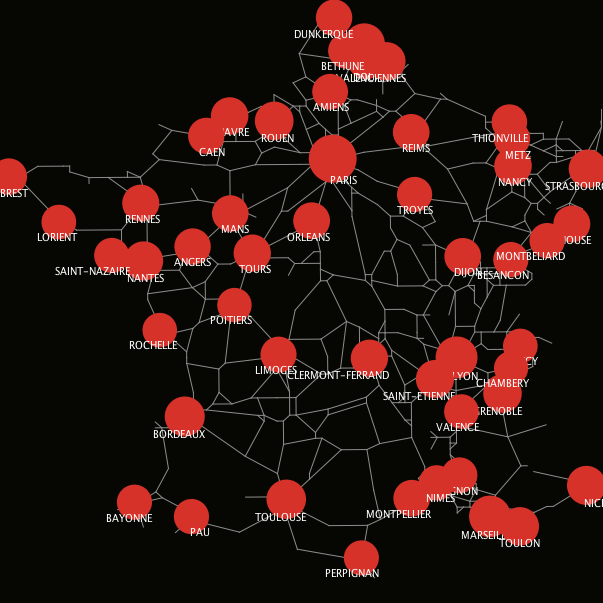
\includegraphics[width=0.48\linewidth]{figures/ex_real_1975.png}
	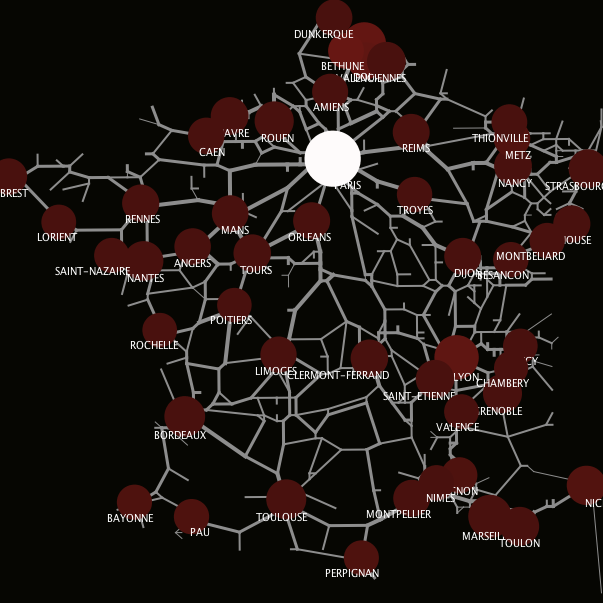
\includegraphics[width=0.48\linewidth]{figures/ex_real_1975_tf_adjusted.png}
	\caption{\textbf{Application of the co-evolution model with a physical network for the French system of cities.} }
\end{figure}
%%%%%%%%%%%%



\subsection{Quantifying hierarchy in systems of cities}


Indicators to understand macroscopic trajectories in simulated systems of cities have been introduced by \cite{raimbault2020unveiling}. They include some related to hierarchy but are not specifically focused on this aspect. We propose now to give a broad set of indicators to capture different dimensions of hierarchy.


\subsubsection{Static quantification of hierarchy}

The most straightforward way to quantify hierarchy is to use Zipf rank-size law, or more generally scaling laws. Let $Y_i$ the variable for which the hierarchy is estimated. Assuming $i$ is ordered in decreasing order, the OLS estimation of $\log \left(Y_i\right) \sim \log \left( i\right)$ gives an estimation of the rank-size slope which is a proxy of hierarchy.

% additional params (complementarity of rank-size and primacy index e.g ~ piecewise linear ?)

The correlation between two hierarchies informs how two dimensions correspond in terms of ranks, and is computed with $r_s\left[X_i,Y_i\right]$ for two variables $X_i,Y_i$ with $r_s$ an estimator of Spearman rank correlation.


\subsubsection{Dynamical indicators}

The rank correlation between initial and final distribution of a variable will measure how much an ordering hierarchy was modified, which is different from the variation of hierarchy given the variations of previous indicators such as the rank-size slope.

Dynamical hierarchy regimes are defined the following way: 
% for PSE
% piecewise linear: which indicator?


\subsubsection{Spatialized indicators}

A spatial non-stationary version of a scaling law would write $Y_i (\vec{x}) \sim \left(\frac{X_i(\vec{x})}{X_0 (\vec{x})}\right)^{\alpha (\vec{x})}$, where $\vec{x}$ is the spatial position and assuming that samples can be defined at each point in space. In practice, a discrete version could be more relevant, for which $\vec{x}_k$ center point are defined, samples consist of points within Thiessen polygons of centers and the exponents are estimated for each center $\alpha (\vec{x}_k)$. Some heuristics should be developed to estimate such a discrete non-parametric scaling law, and remains out of the scope of this paper.



%%%%%%%%%%%%%%%%
\section{Results}


\subsection{Implementation}

The model is implemented in NetLogo \cite{tisue2004netlogo}, which is a good compromise between performance and interactivity, the former being necessary with a model with such a spatialized network. 


\subsection{Hierarchy patterns}

% grid explo, compare virtual/physical
% - compare abstract network with physical (Theo Quant results) (not necessary calibration here? )

%%%%%%%%%%%%%%
\begin{figure}
\centering
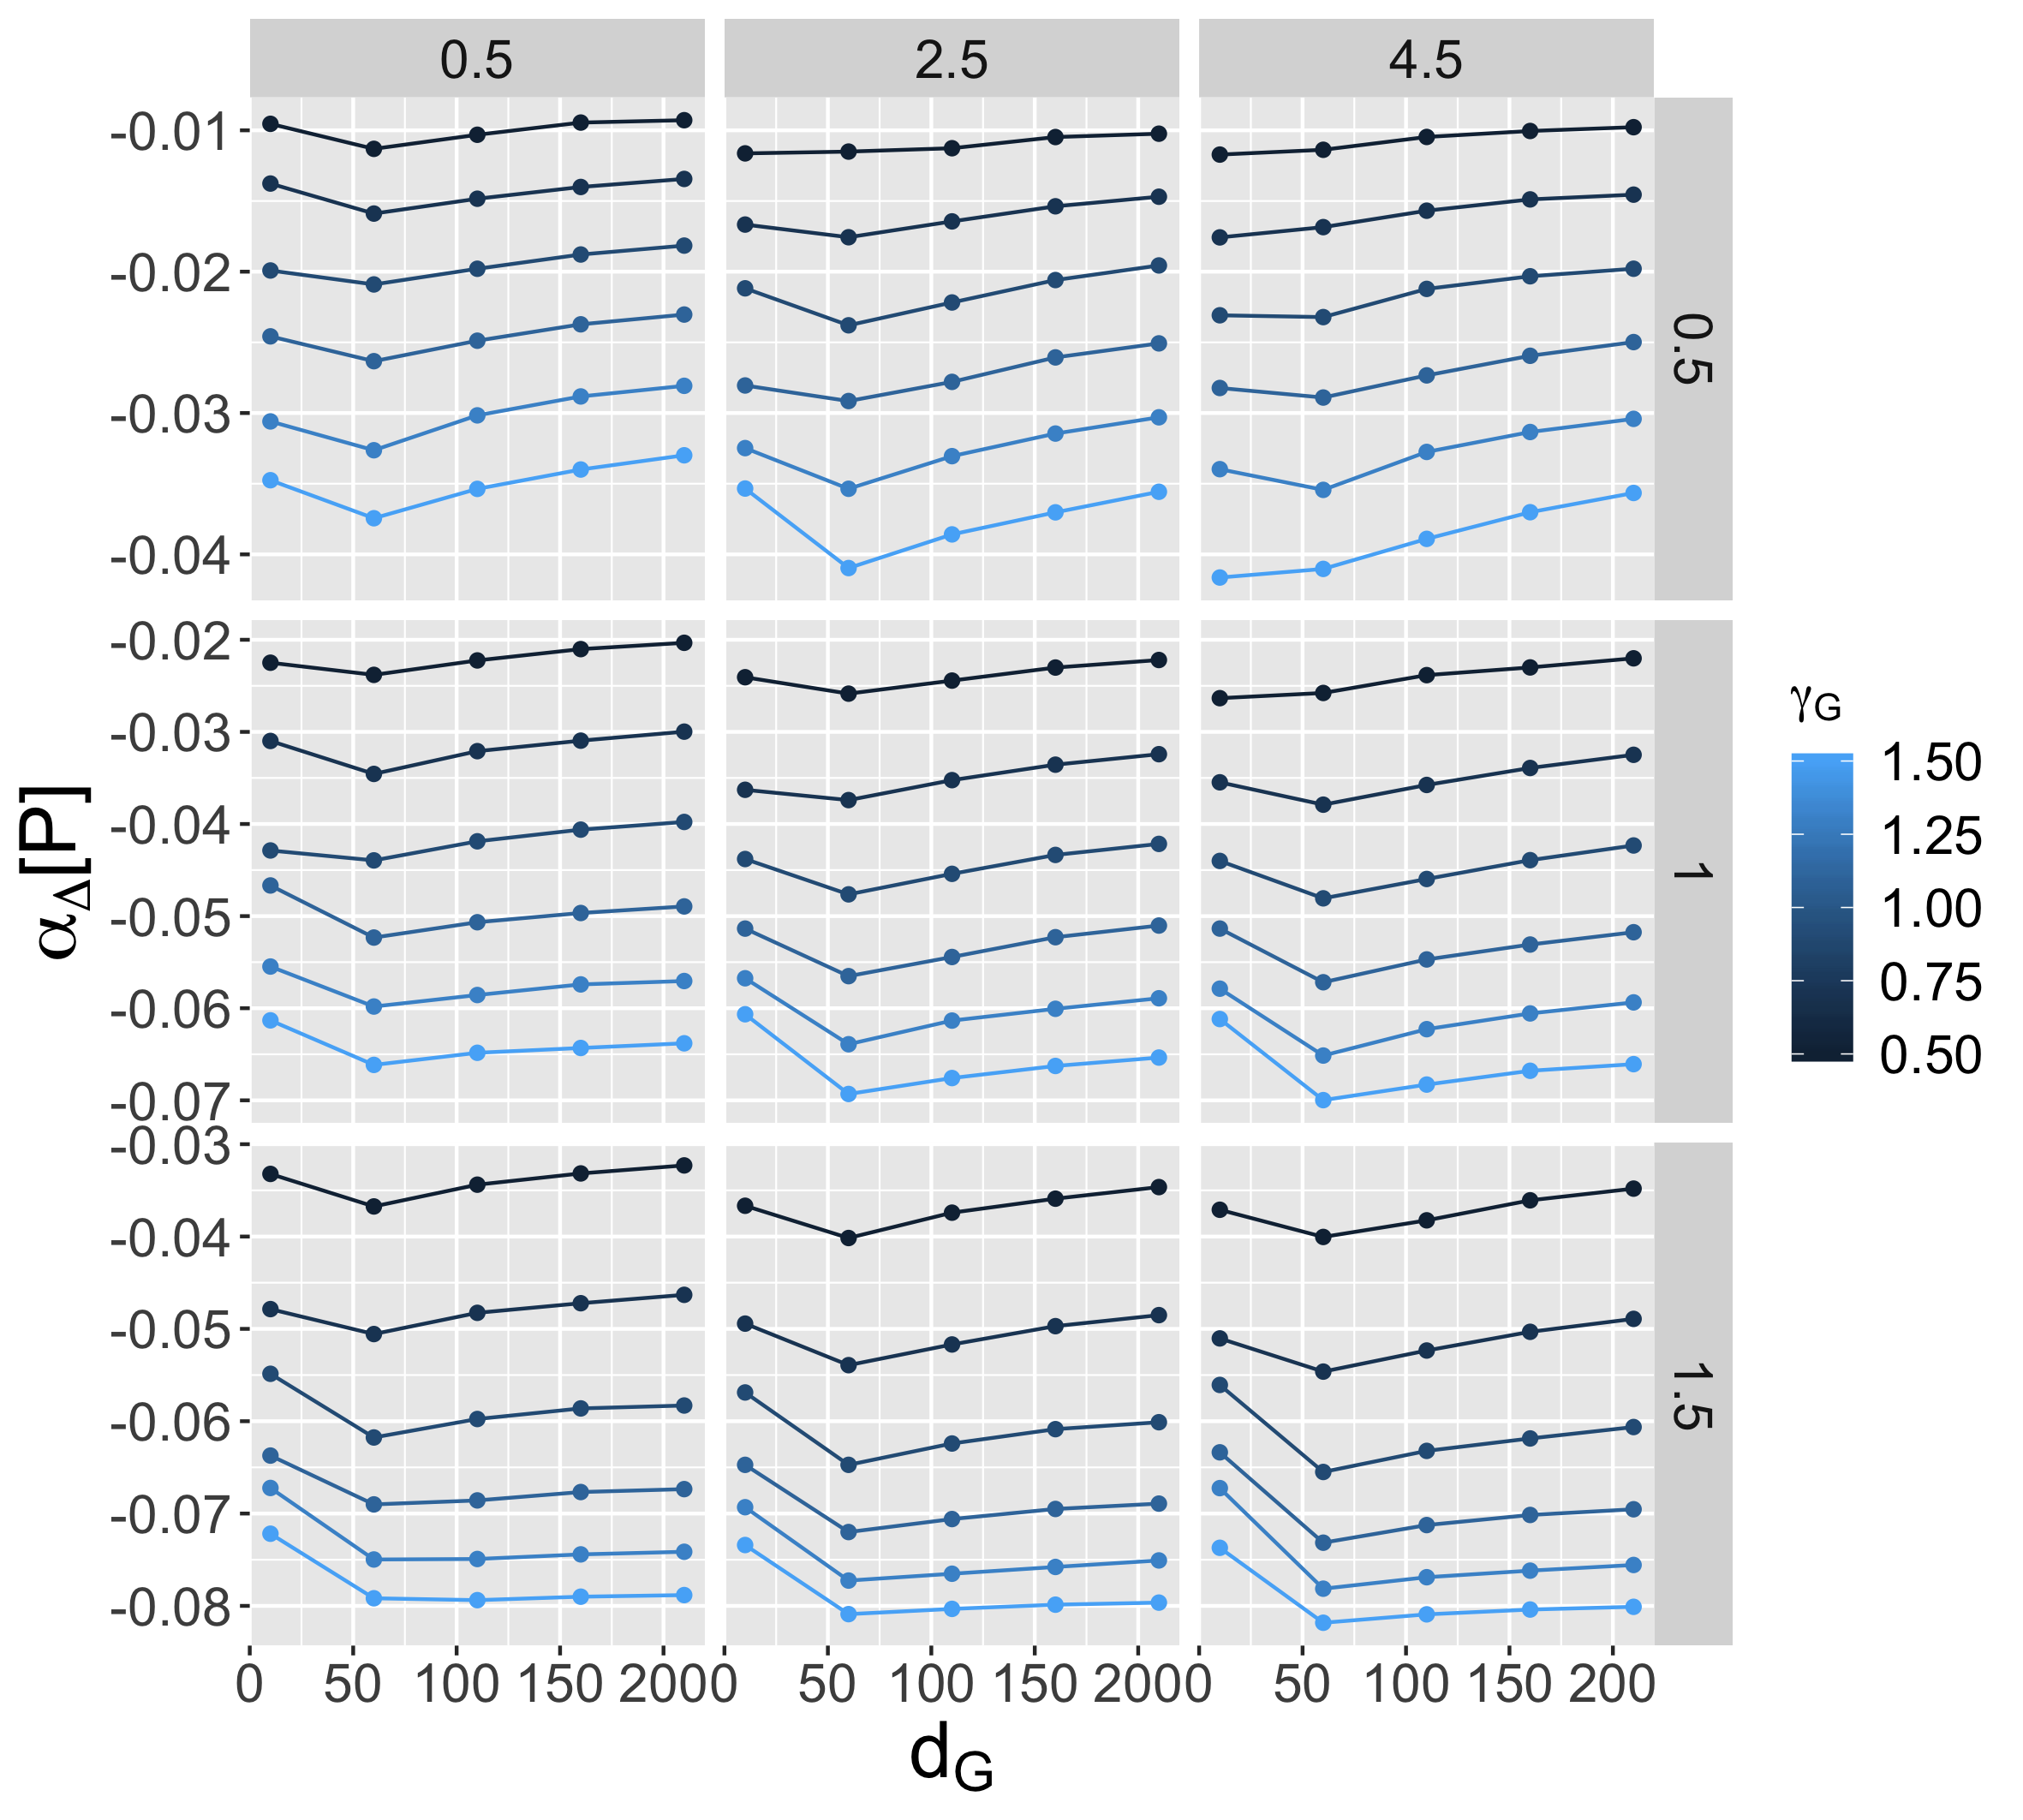
\includegraphics[width=0.48\linewidth]{figures/hierarchiesPopAlpha_nwExp1_wG0_001_xgravityDecay_colgravityGamma_facetsynthRankSize-nwThreshold.png}
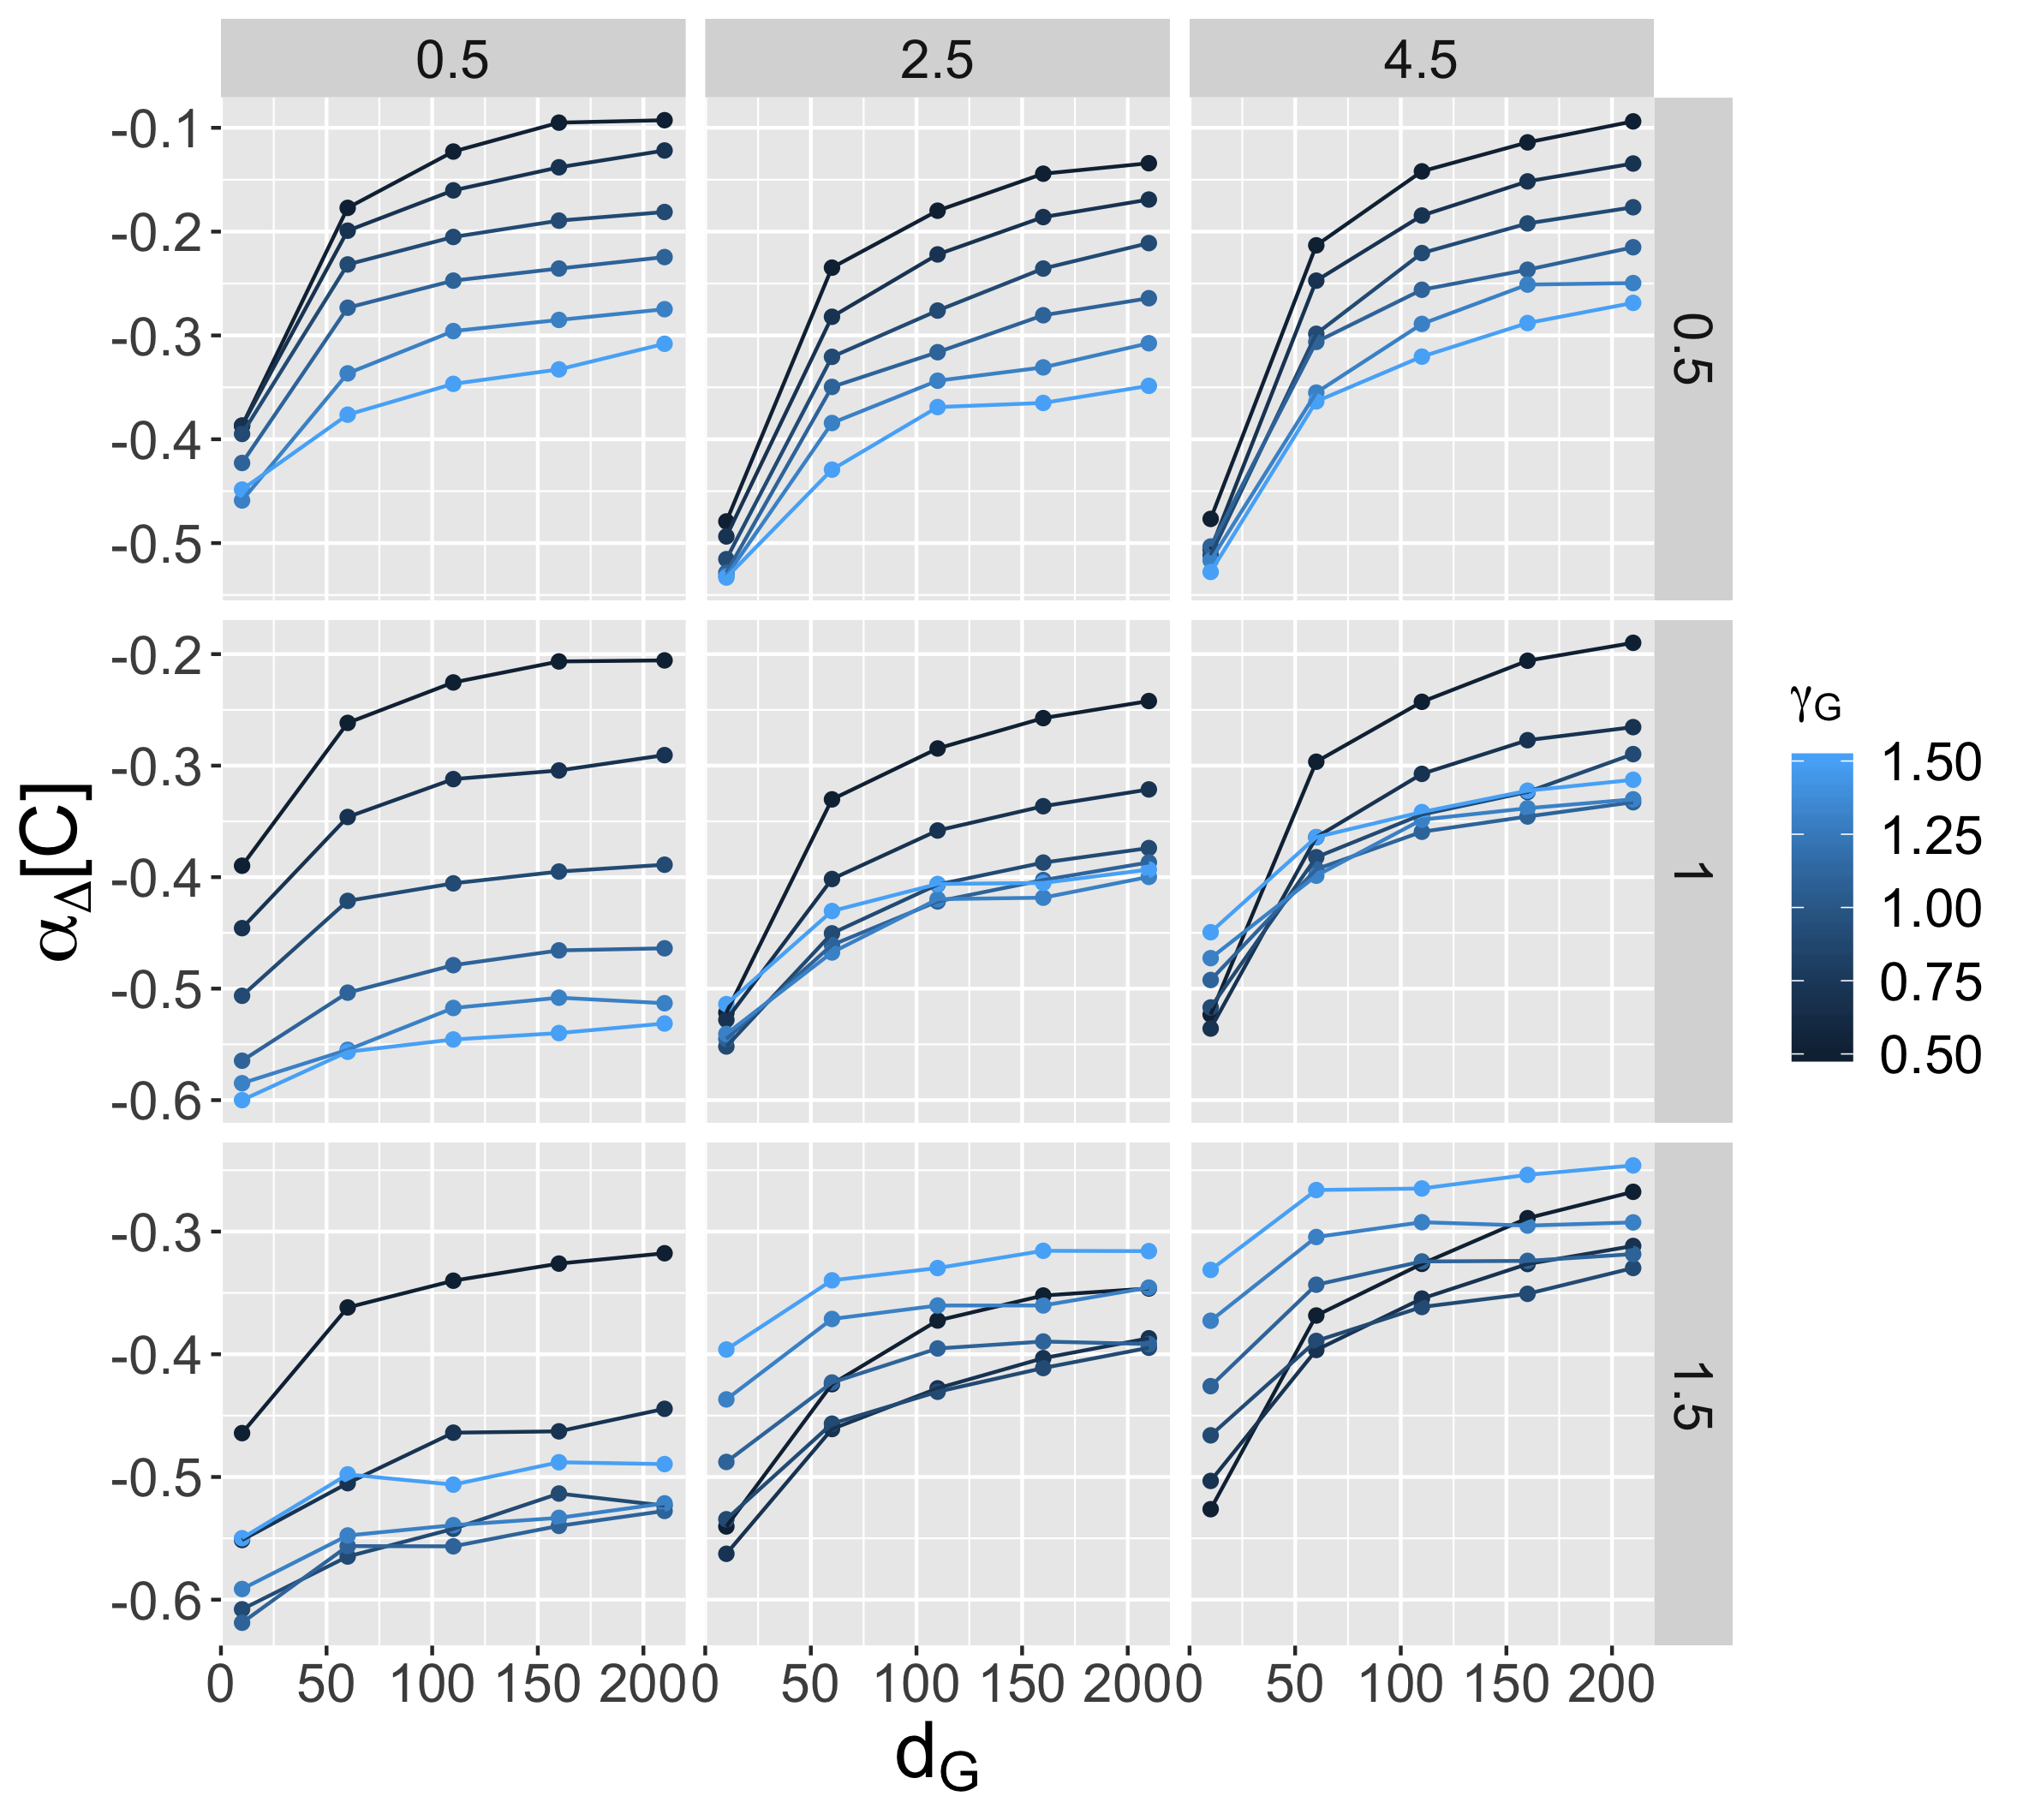
\includegraphics[width=0.48\linewidth]{figures/hierarchiesClosenessAlpha_nwExp1_wG0_001_xgravityDecay_colgravityGamma_facetsynthRankSize-nwThreshold.png}\\
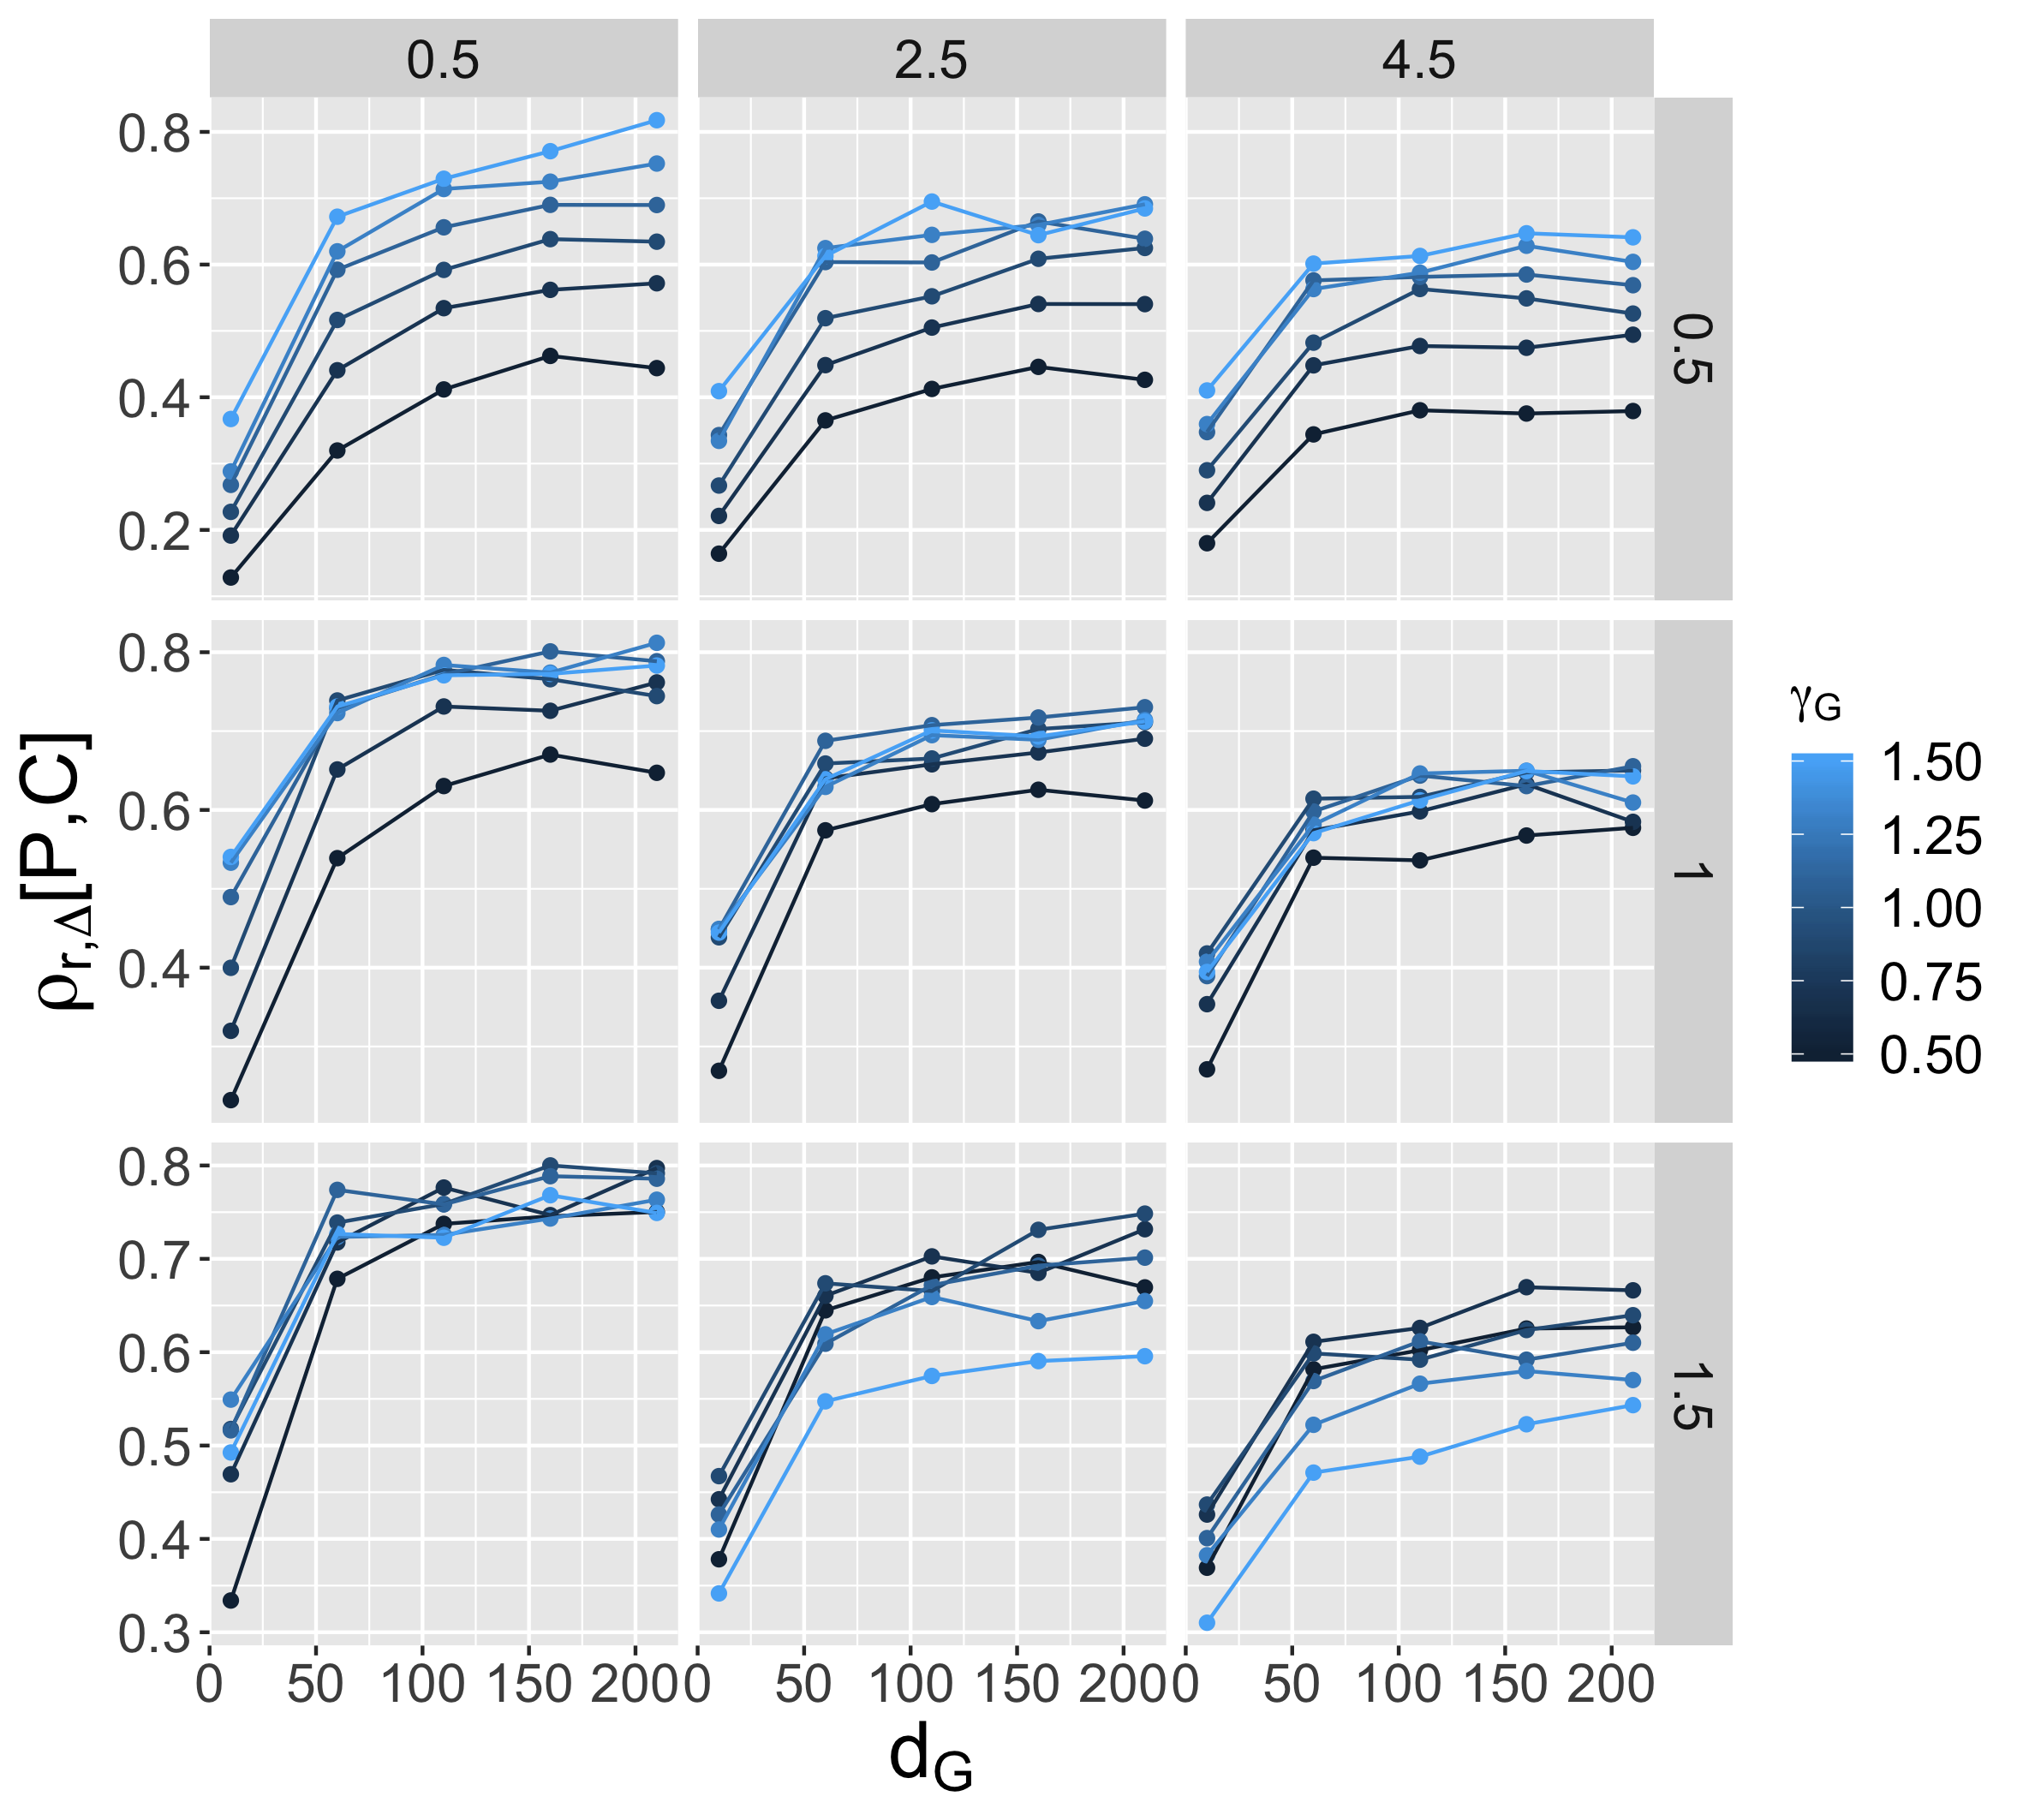
\includegraphics[width=0.48\linewidth]{figures/rankCorrsPopCloseness_nwExp1_wG0_001_xgravityDecay_colgravityGamma_facetsynthRankSize-nwThreshold.png}
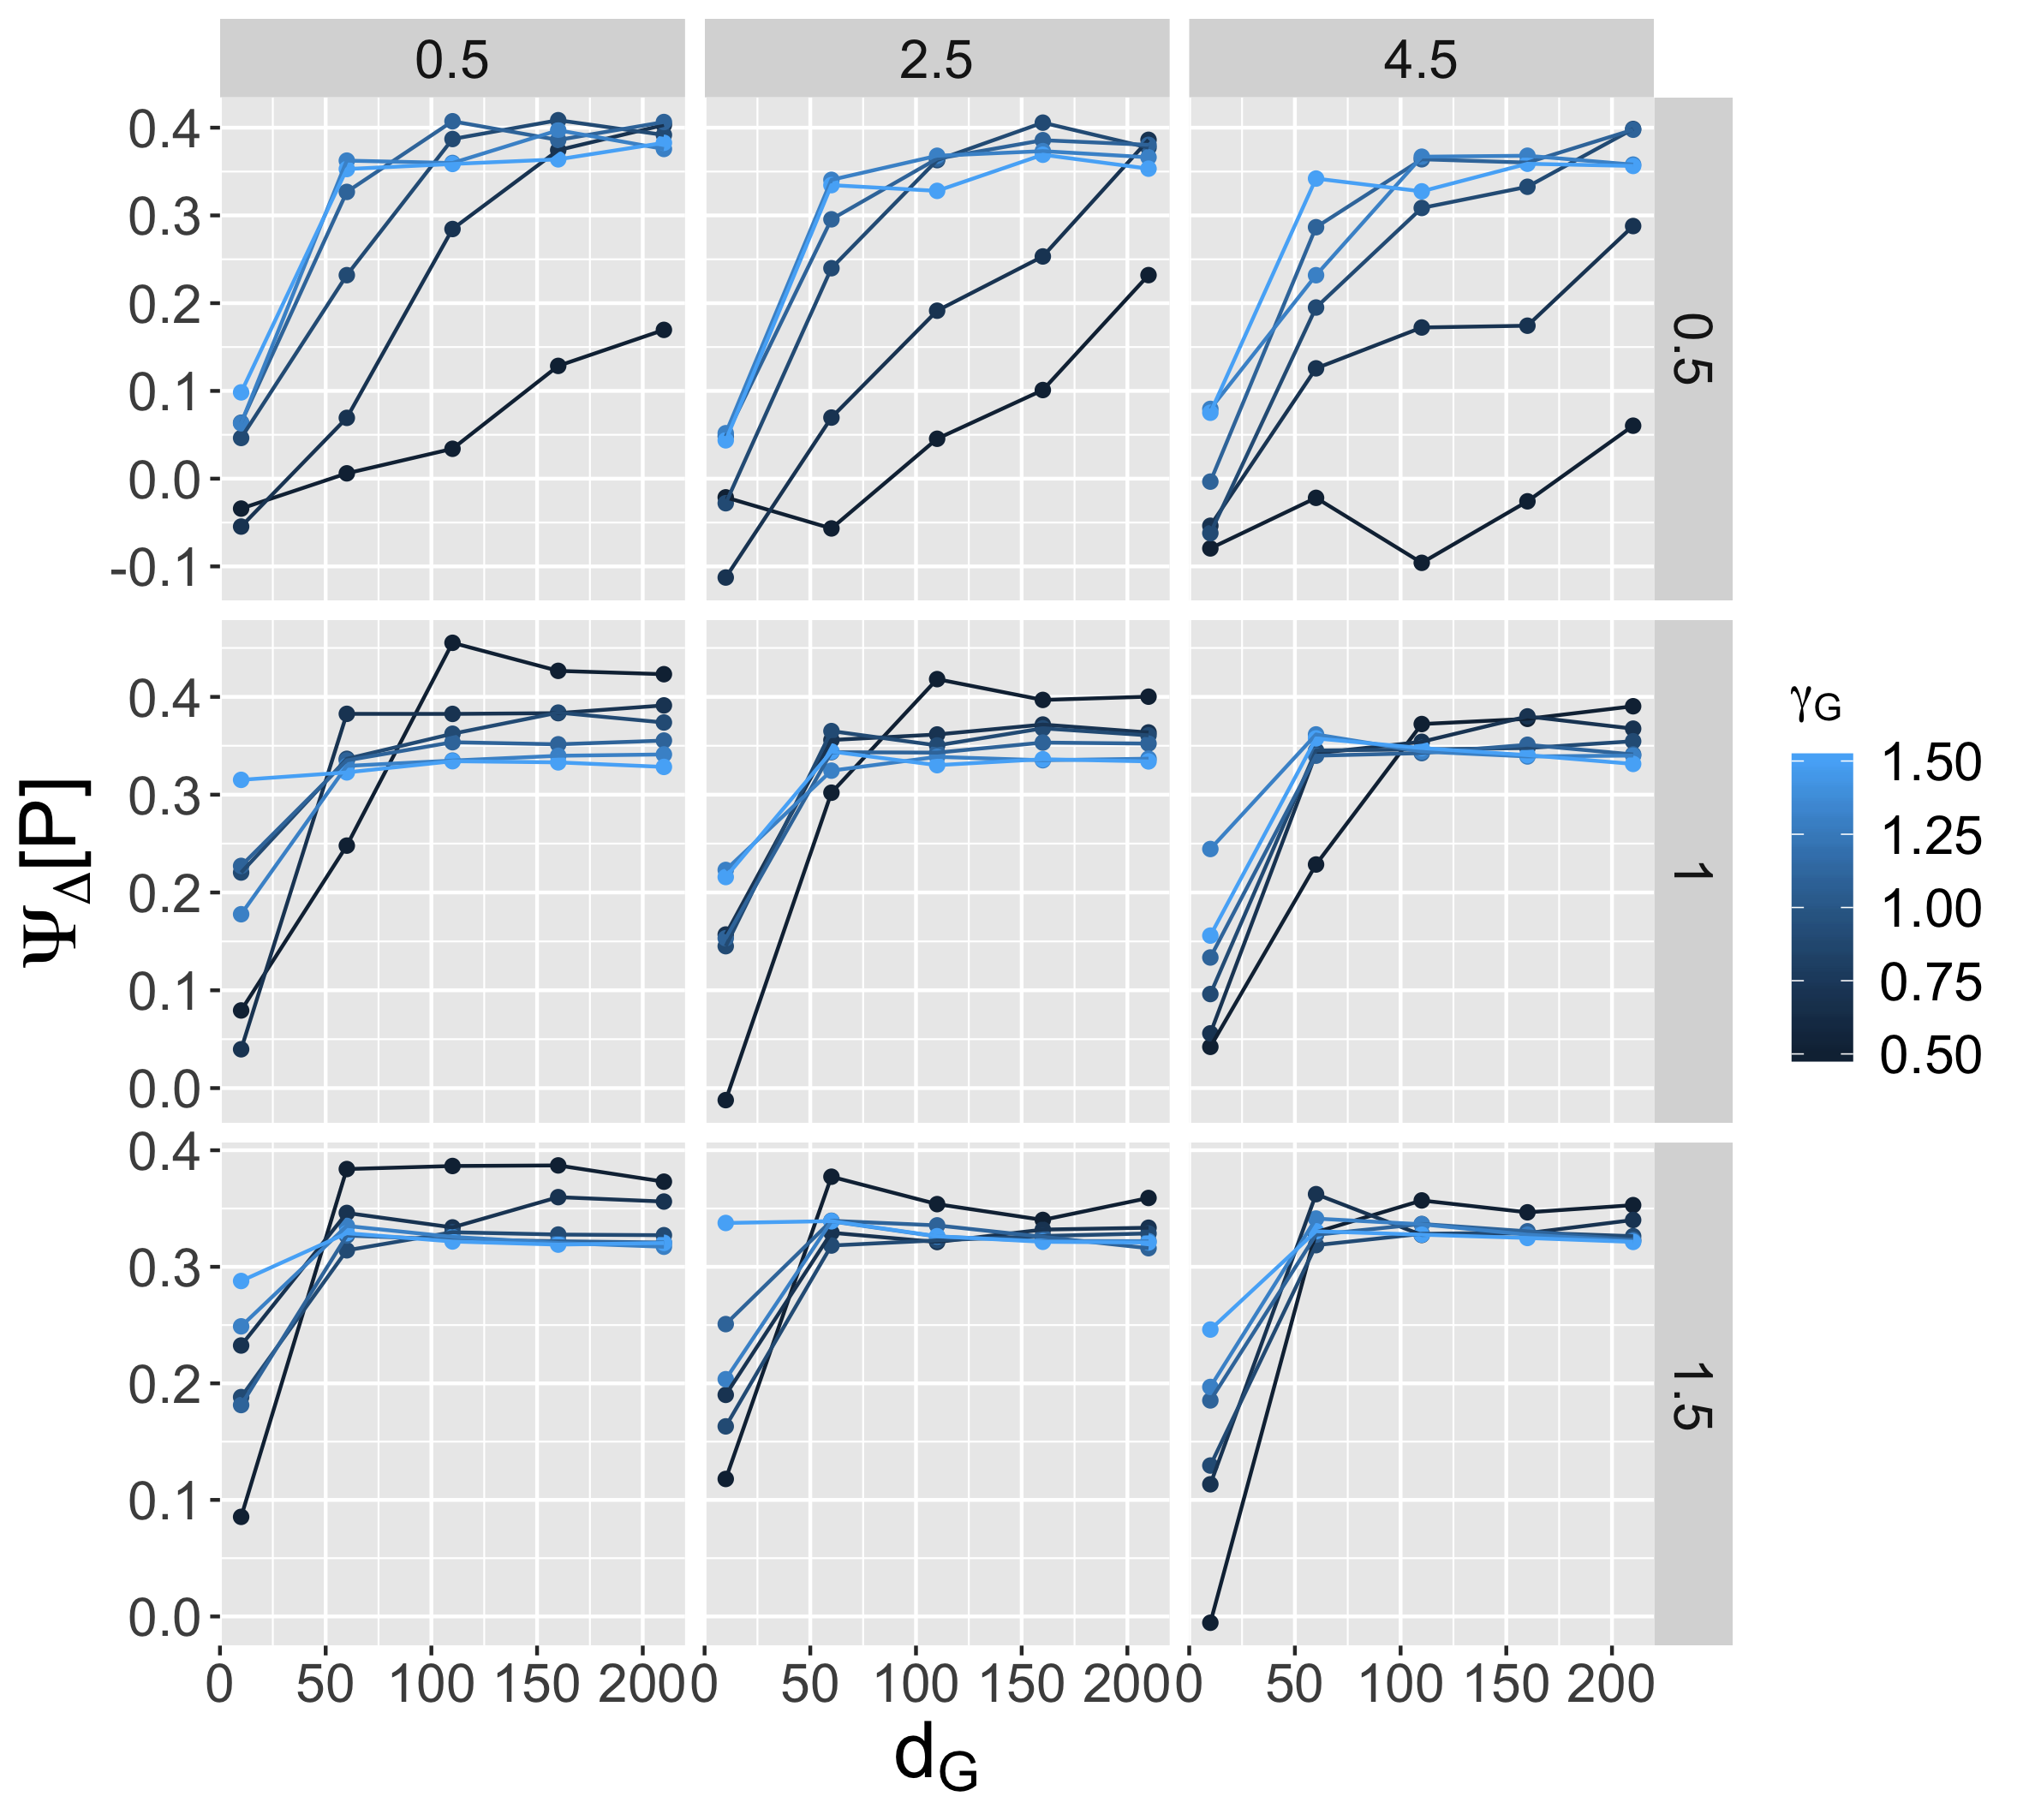
\includegraphics[width=0.48\linewidth]{figures/segHierarchiesPopPsi_nwExp1_wG0_001_xgravityDecay_colgravityGamma_facetsynthRankSize-nwThreshold.png}
\caption{\textbf{Patterns of hierarchy in the model with a virtual network.} \textit{(Top Left)} Difference in the rank-size exponent between final time and initial time, }
\end{figure}
%%%%%%%%%%%%%%

%%%%%%%%%%%%%%
\begin{figure}
\centering
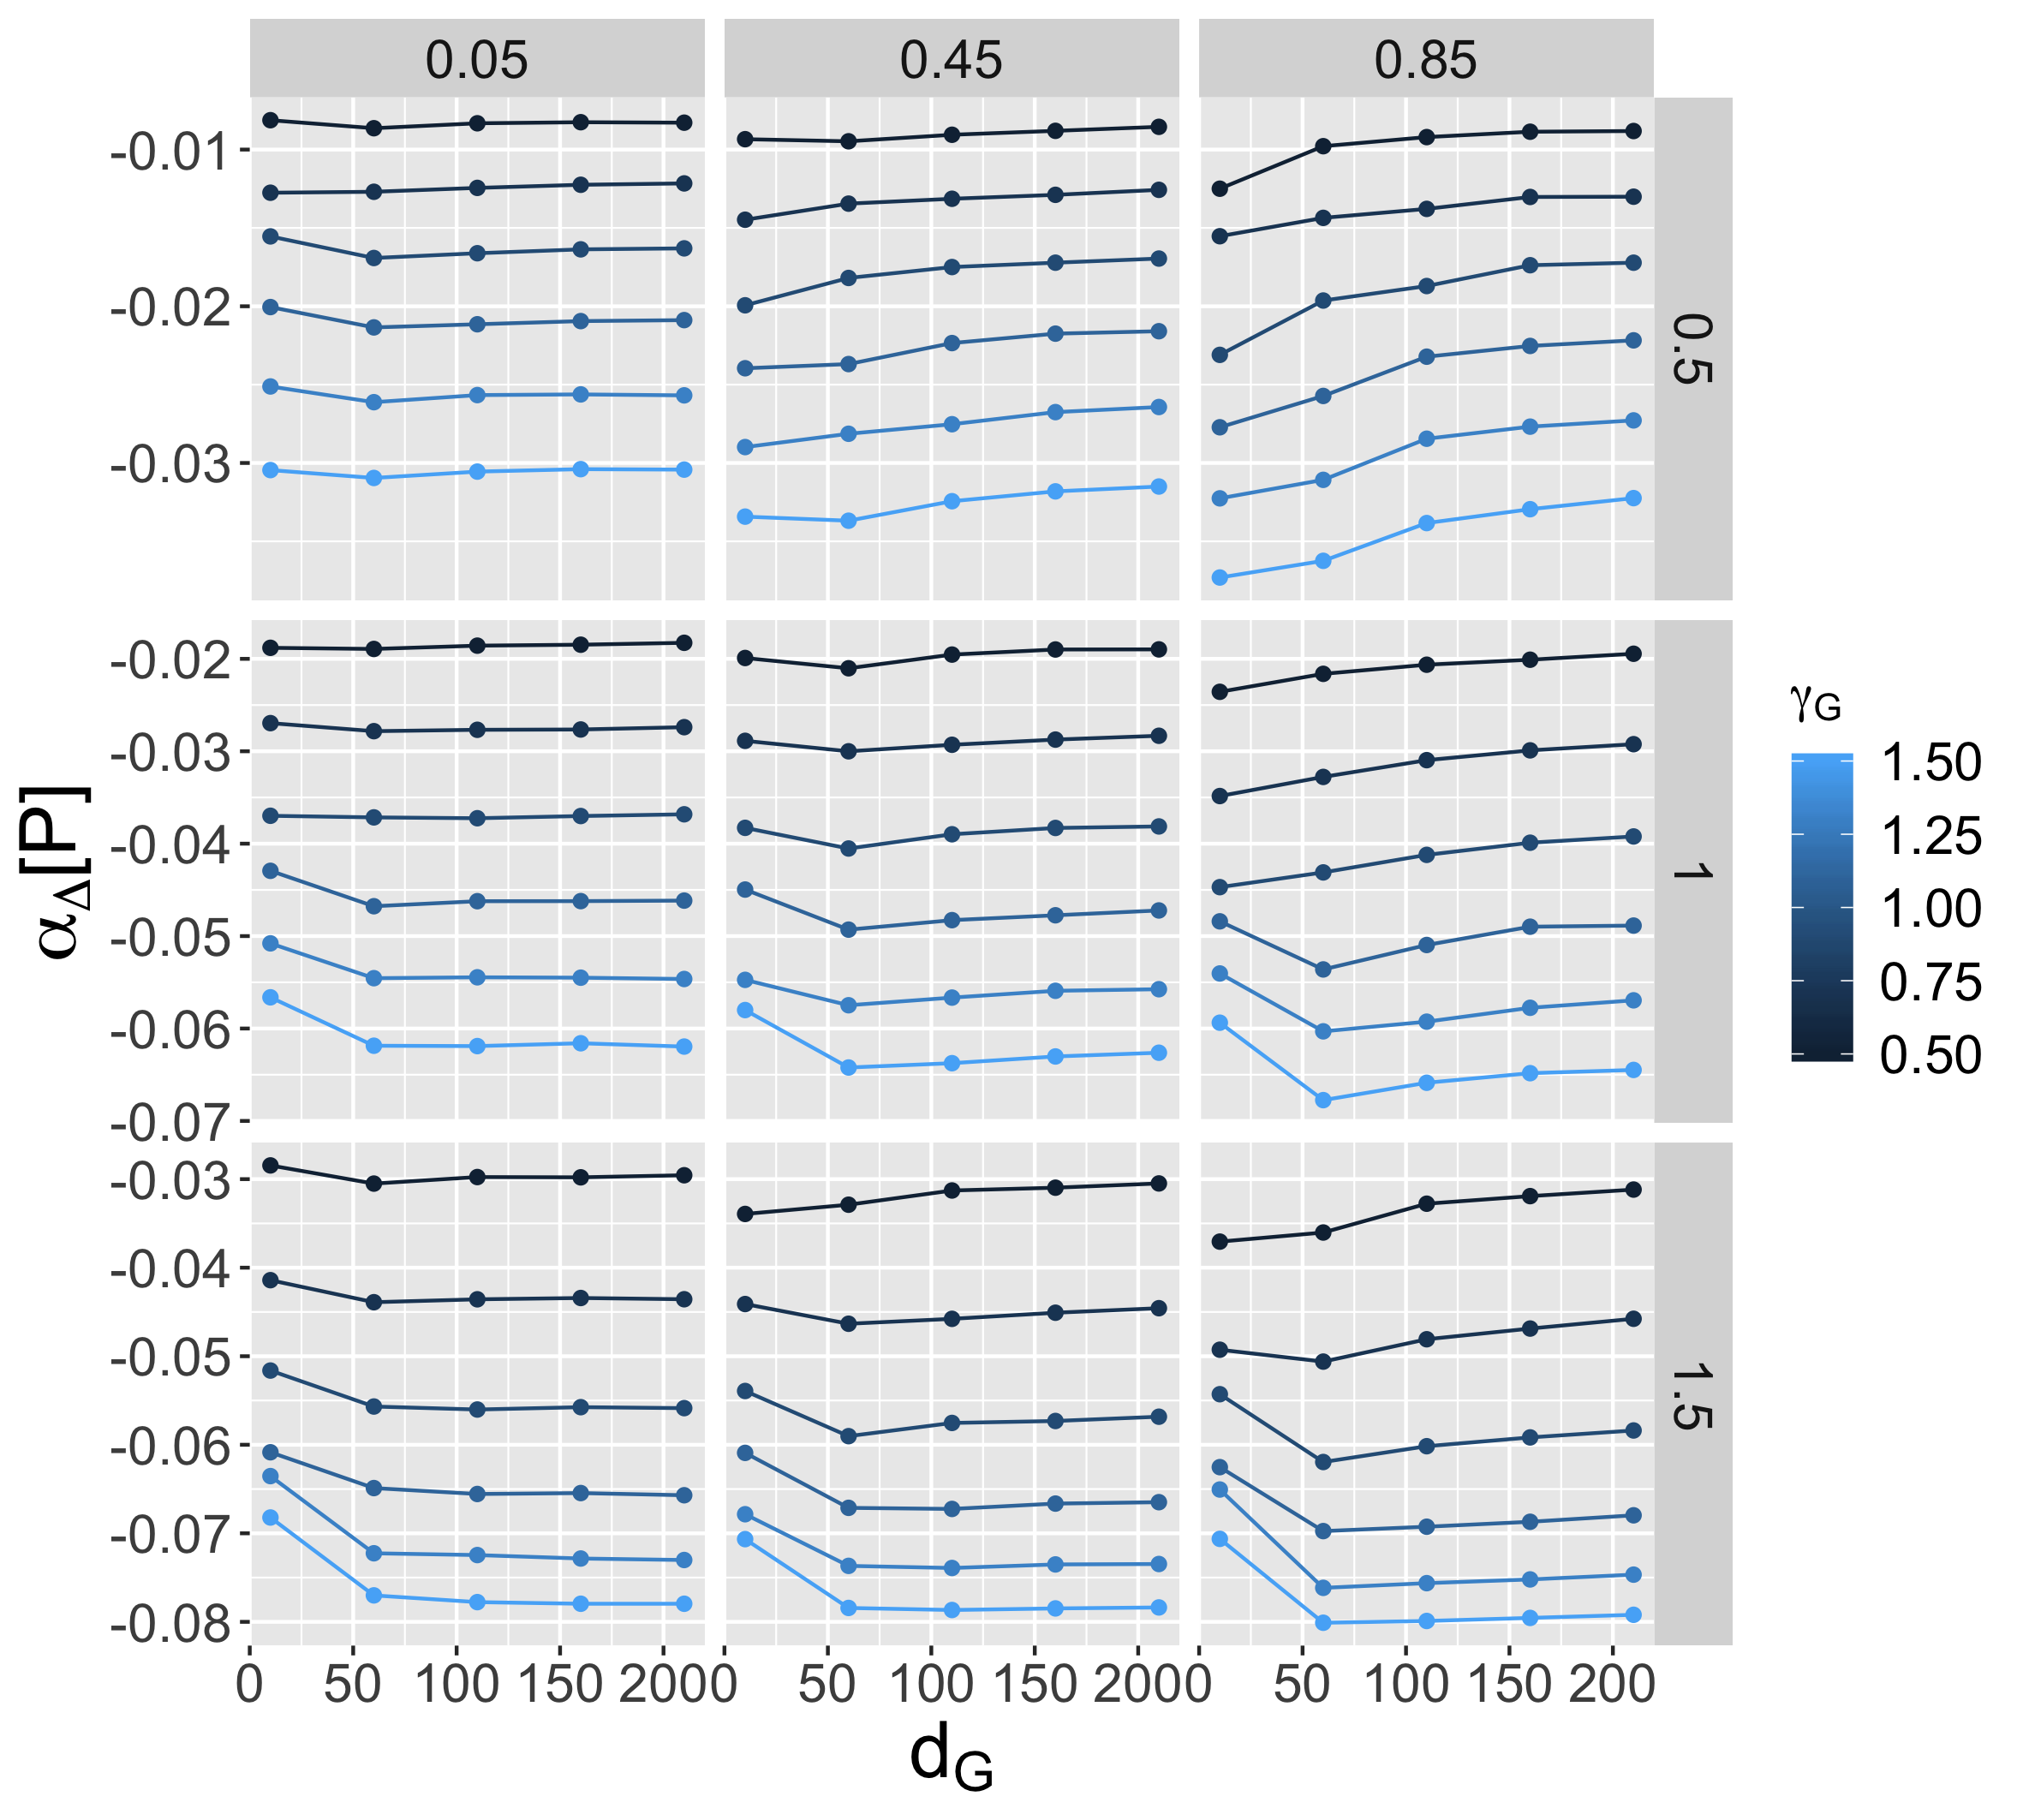
\includegraphics[width=0.48\linewidth]{figures/hierarchiesPopAlpha_nwExp1_wG0_001_xgravityDecay_colgravityGamma_facetsynthRankSize-nwPhysQuantile.png}
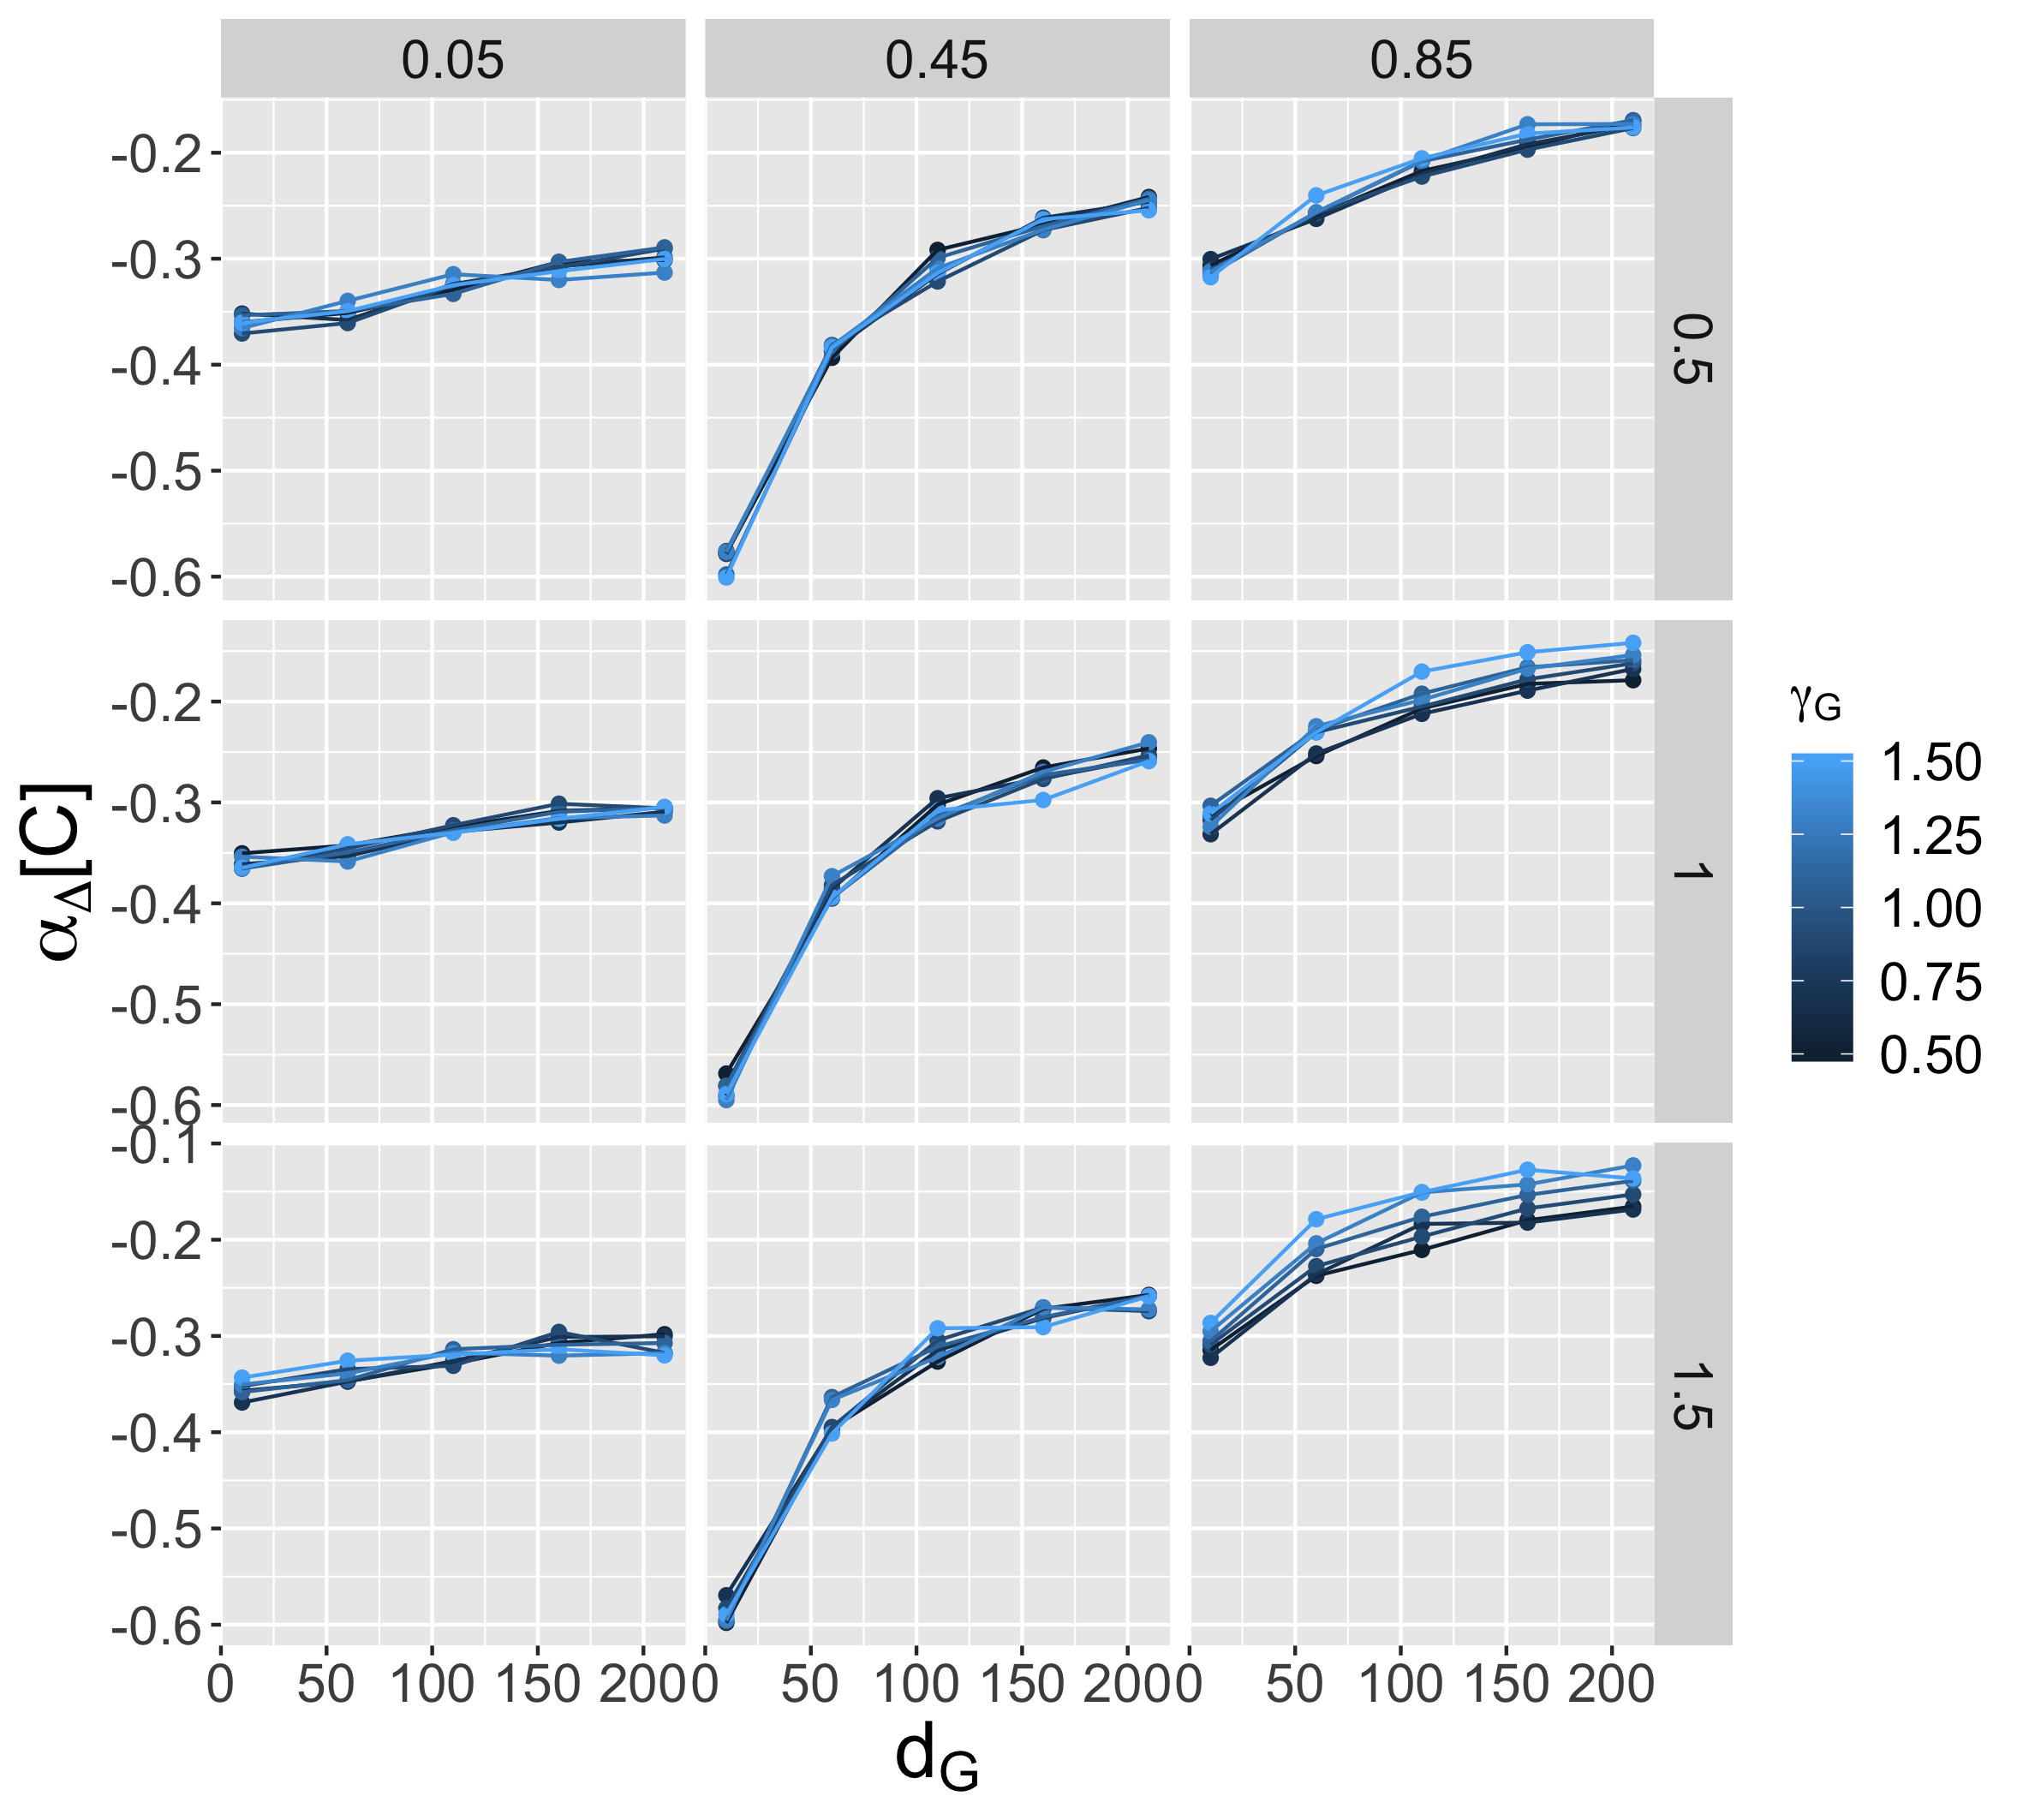
\includegraphics[width=0.48\linewidth]{figures/hierarchiesClosenessAlpha_nwExp1_wG0_001_xgravityDecay_colgravityGamma_facetsynthRankSize-nwPhysQuantile.png}\\
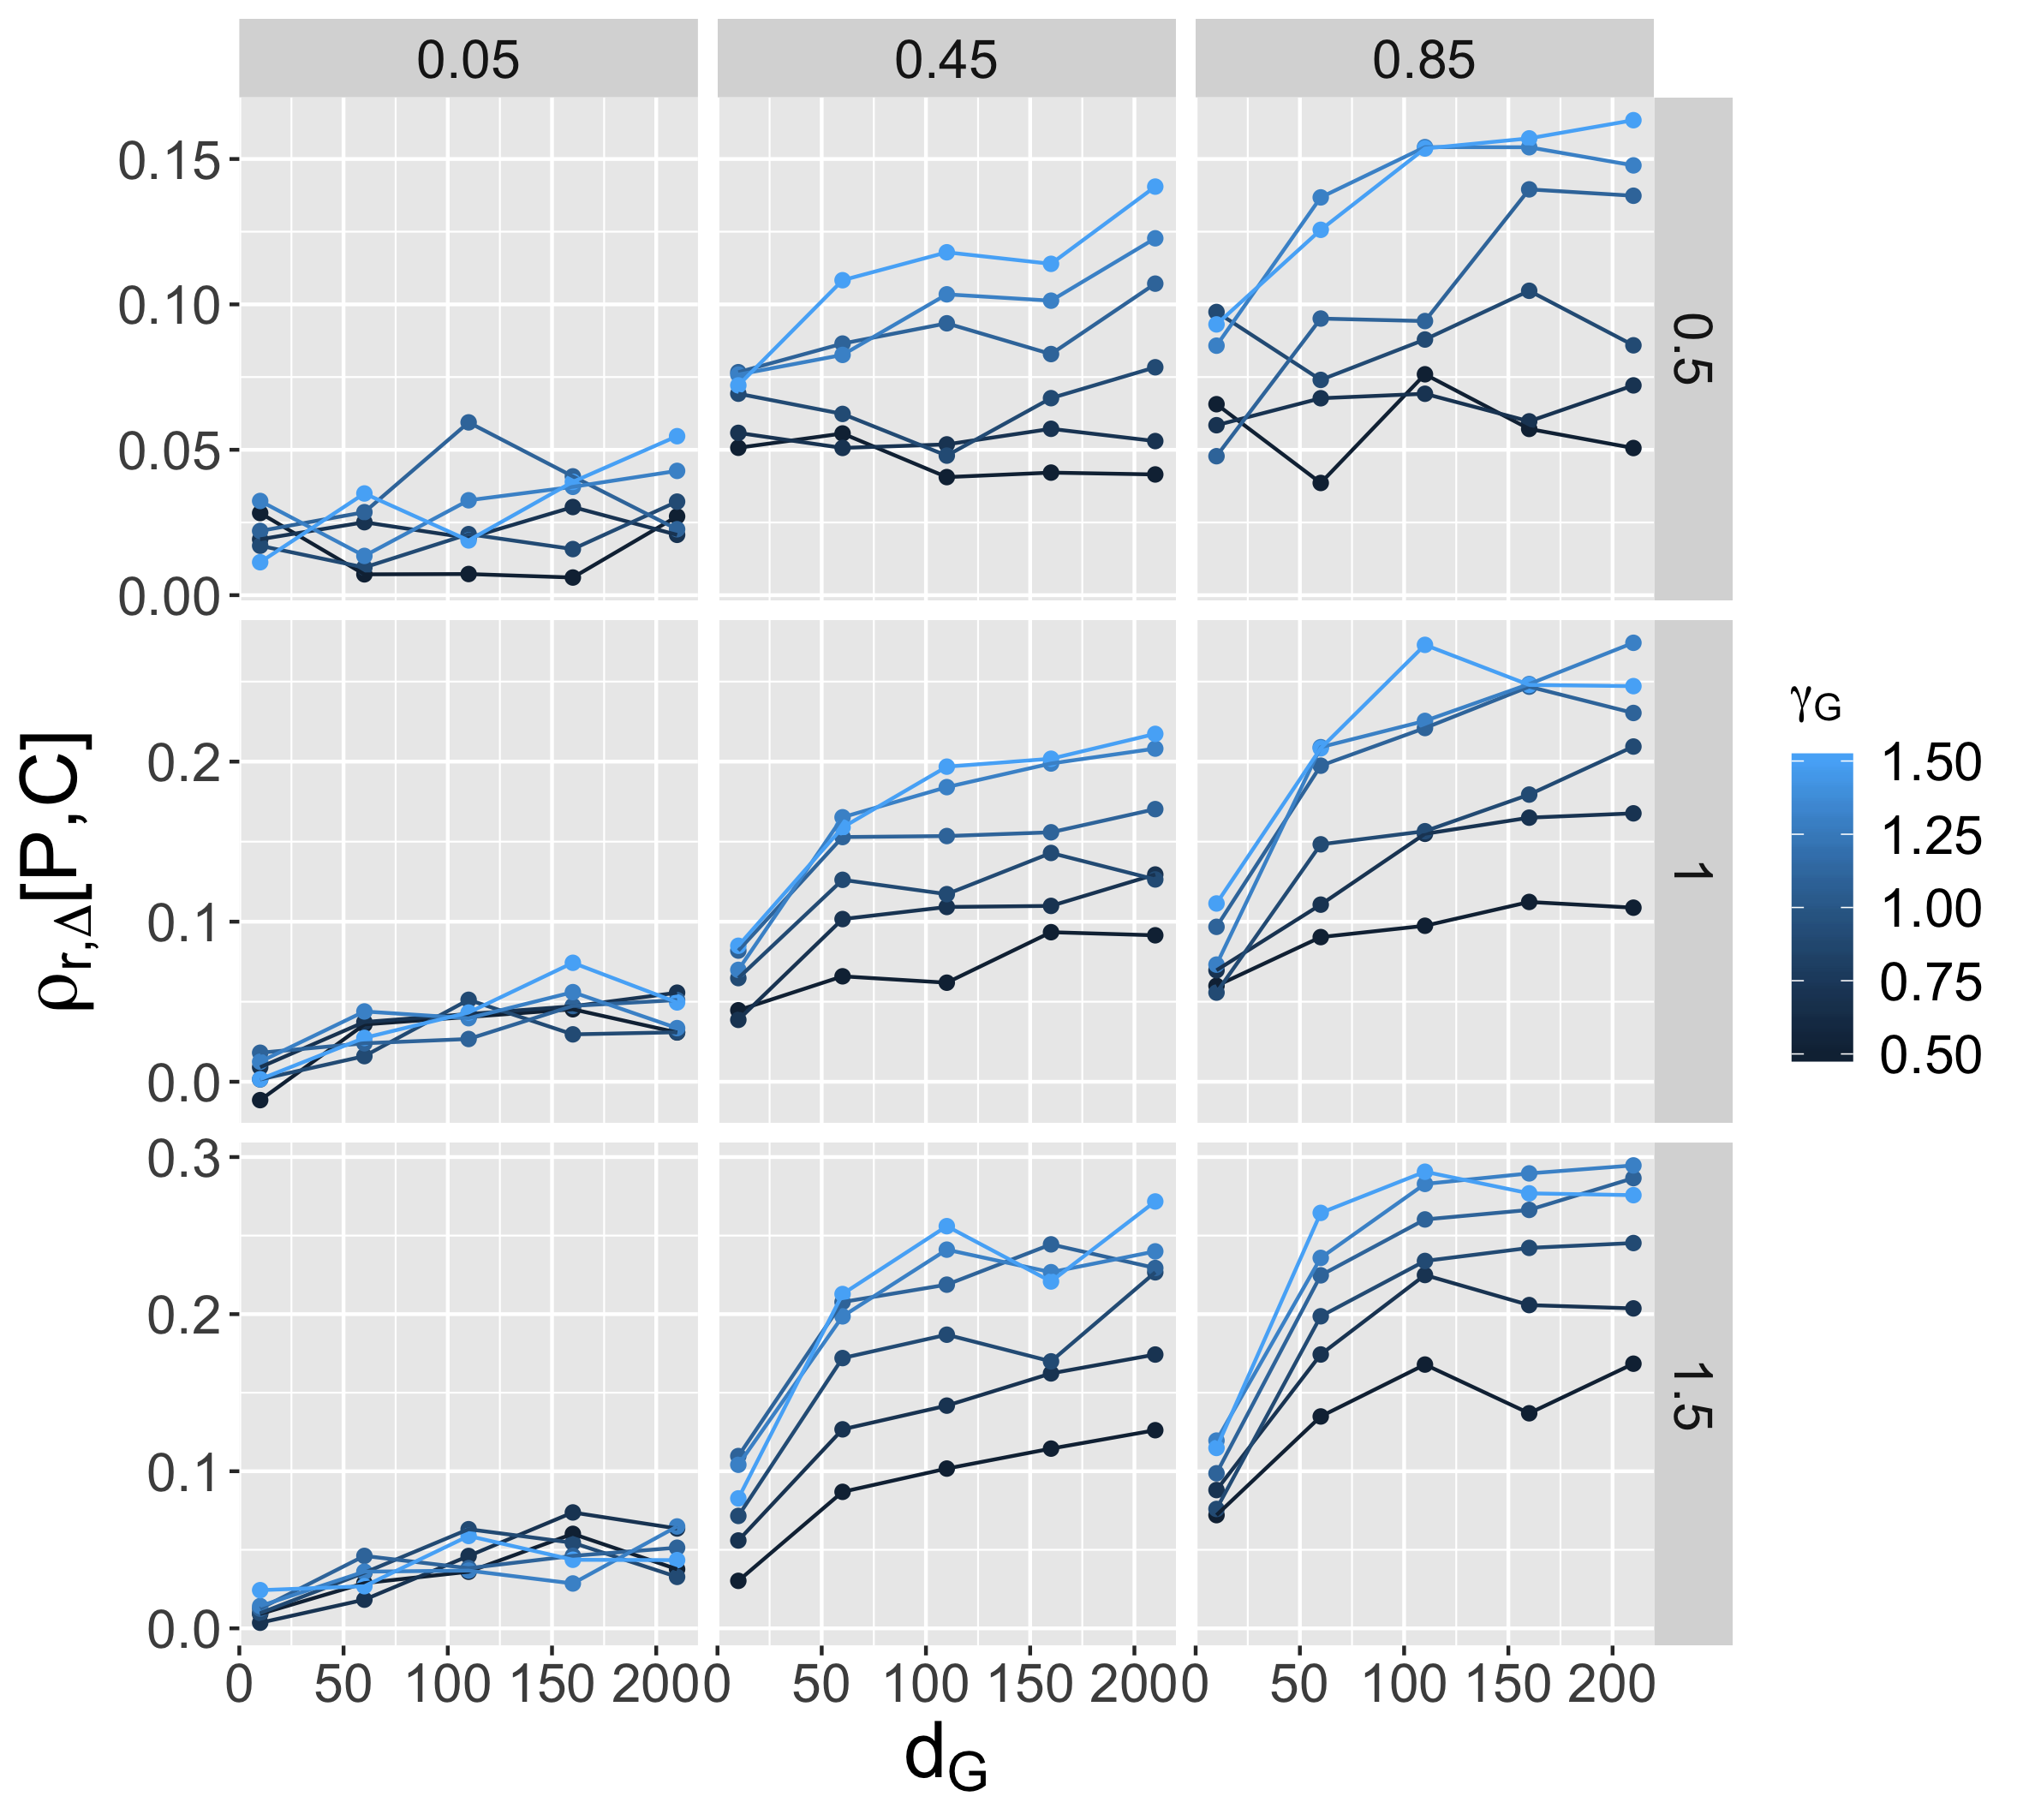
\includegraphics[width=0.48\linewidth]{figures/rankCorrsPopCloseness_nwExp1_wG0_001_xgravityDecay_colgravityGamma_facetsynthRankSize-nwPhysQuantile.png}
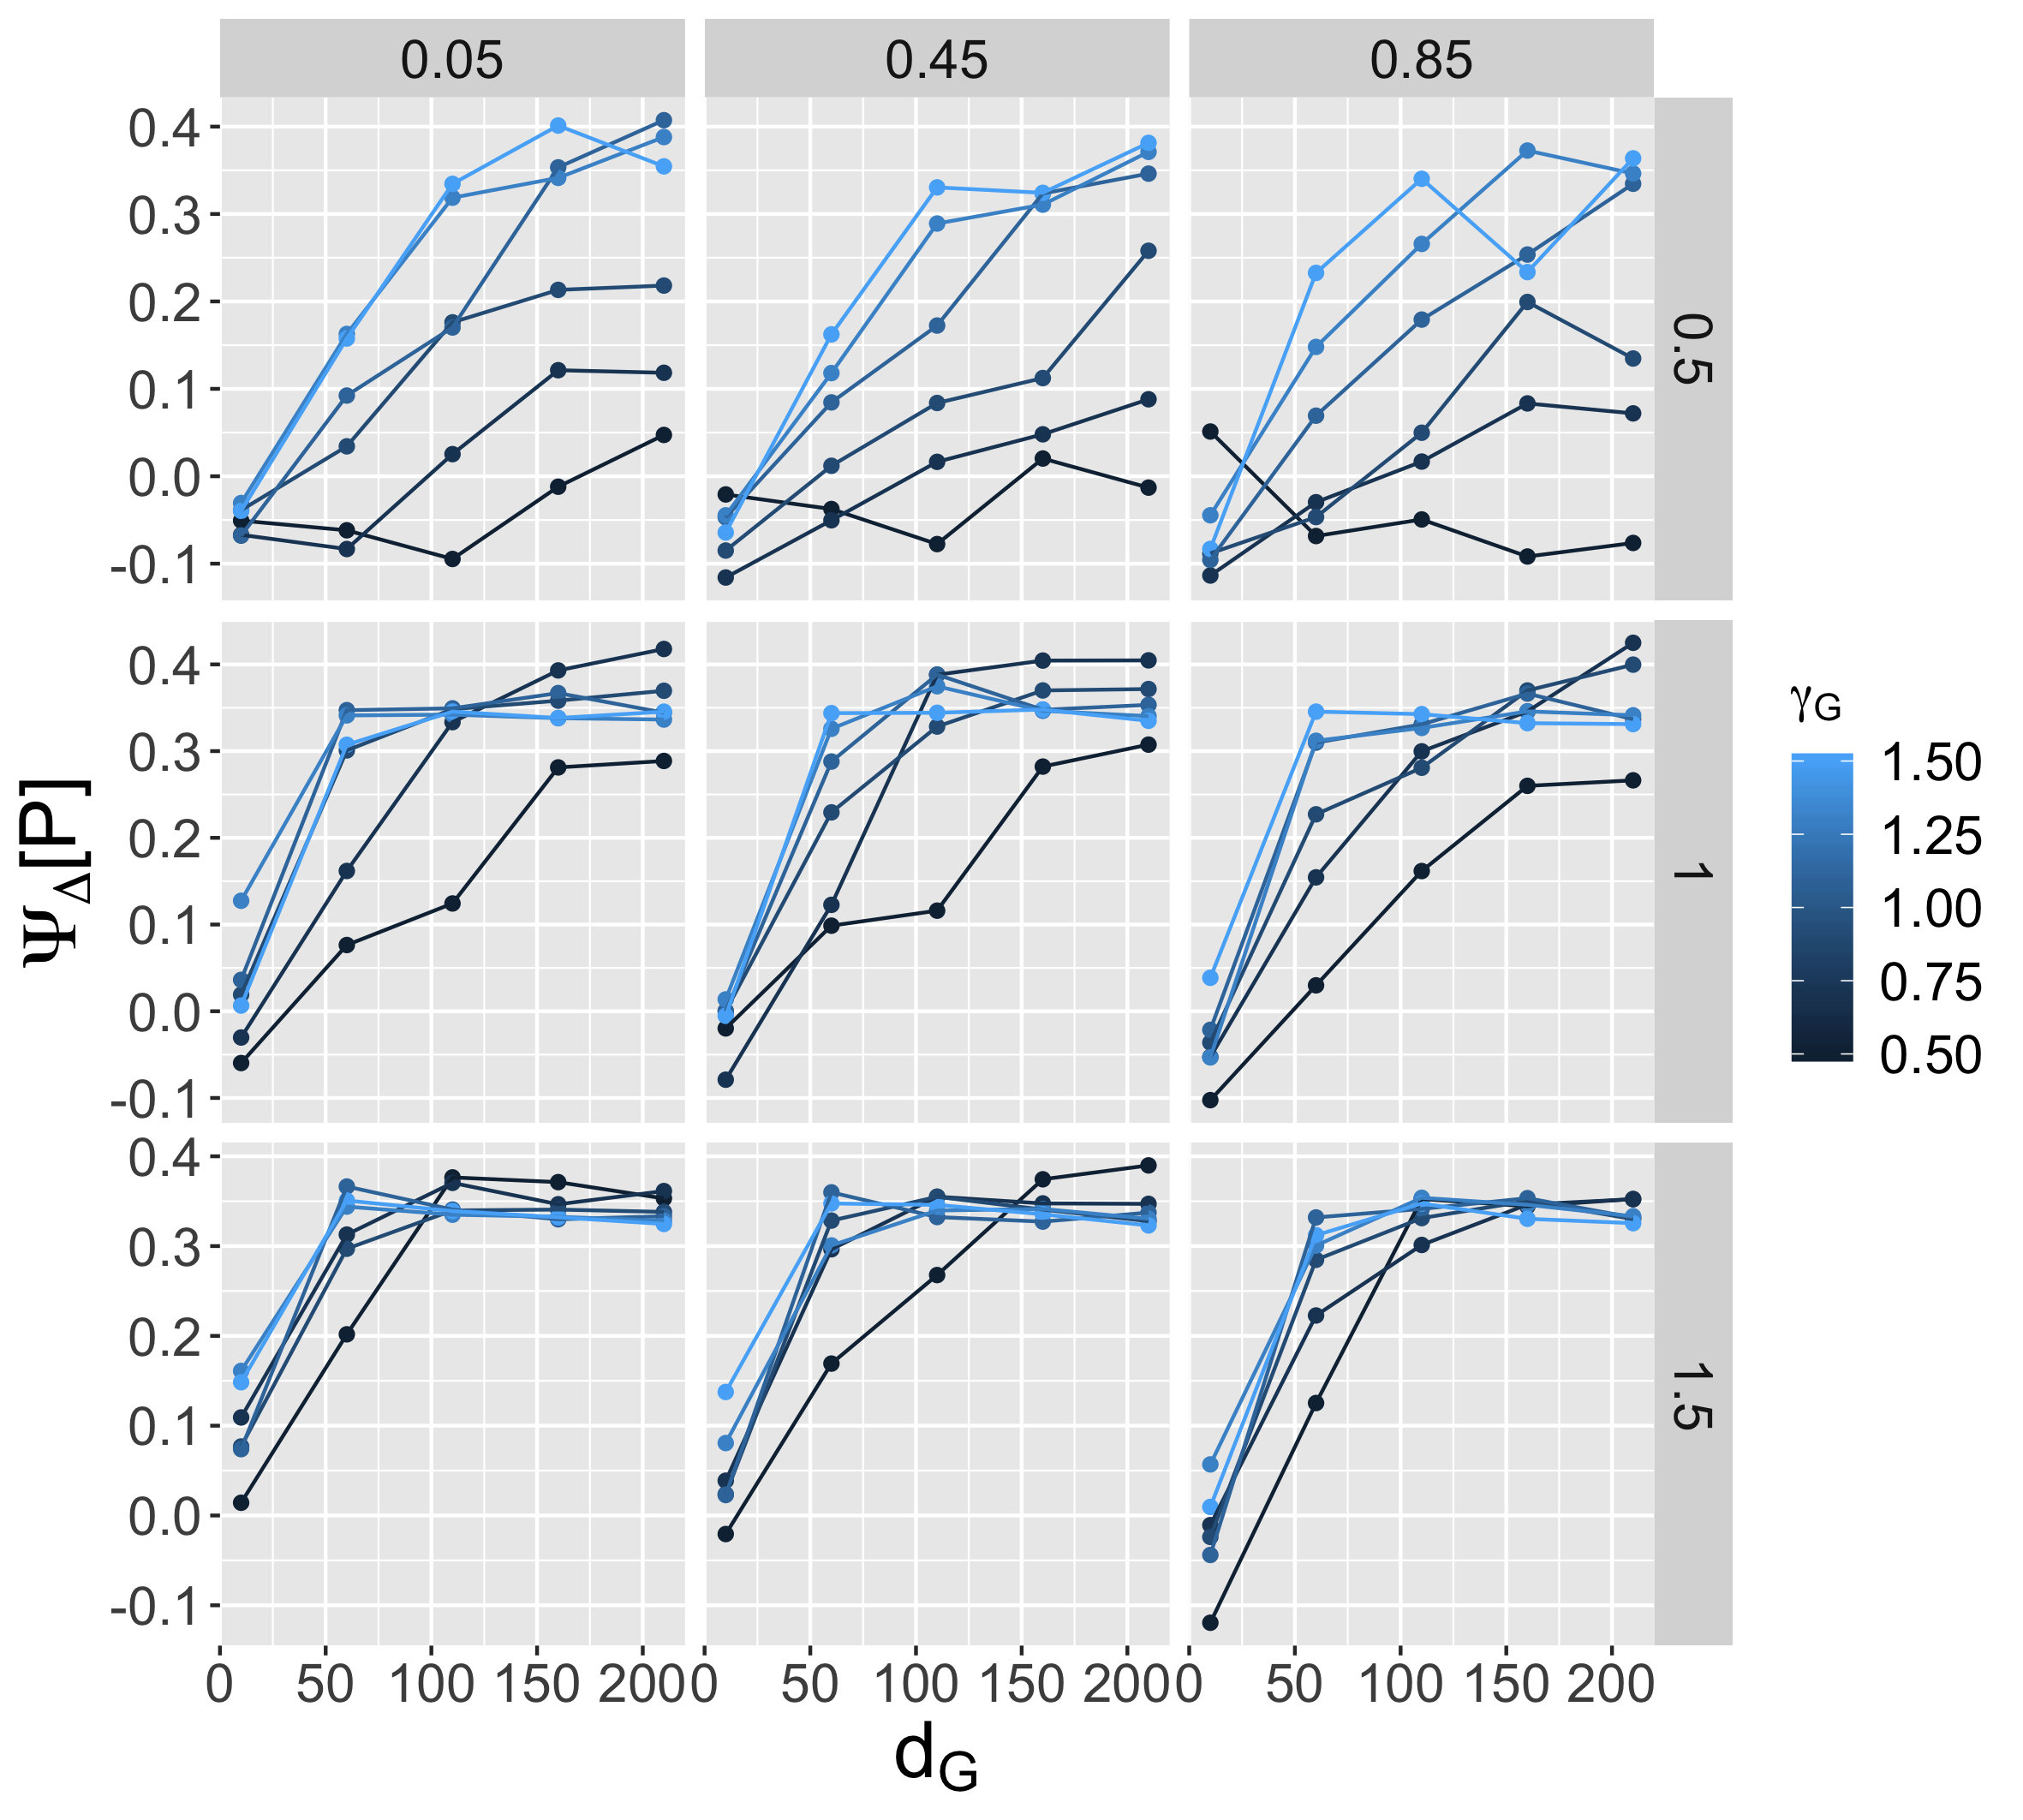
\includegraphics[width=0.48\linewidth]{figures/segHierarchiesPopPsi_nwExp1_wG0_001_xgravityDecay_colgravityGamma_facetsynthRankSize-nwPhysQuantile.png}
\caption{\textbf{Patterns of hierarchy in the model with a physical network.} \textit{(Top Left)}  }
\end{figure}
%%%%%%%%%%%%%%









\subsection{Hierarchy regimes}

% - PSE targeted on different regimes (dynamical ?) of hierarchy => piecewise linear fitting? 







%%%%%%%%%%%%%%%%
\section{Discussion}



\subsection{Results on co-evolution and hierarchies}

% what do we learn in this particular context ?
% - teachings on the role of self-reinforcement




\subsection{Developments}

%\subsection{Spatial hierarchical niches}
% possible experiment: optim algo to isolate optimal fitting niches; find typical niche size when varying parameters
% (out of the scope / development of algo in itself)


\subsection{Theoretical perspective}

% ~ disc from jig ?

% \textbf{Proposition : } \textit{les hiérarchies, au sens d'imbrication de sous-systèmes à de multiples niveaux, sont endogènes aux systèmes complexes}
% des structures ``hiérarchiques'' au sens commun (structure de dépendance rigide et arborescente) sont simples et ni adaptatives ni résilientes
% le concept de hiérarchie ne peut être considéré comme exogène et totalement déconstruit
% pour l'aide à la décision, des utopies réductionnistes en horizontalité complète s'opposent aux théories de la complexité
% question ouverte (reflexive): endogènes \textit{aux systèmes} ou aux \textit{théories et modèles des systèmes} ?
%\textbf{Des approches multi-scalaires intégratives pour des gouvernances territoriales soutenables \cite{rozenblat2018conclusion} doivent prendre en compte la complexités des hiérarchies.}





%%%%%%%%%%%%%%%%
\section{Conclusion}




\bibliographystyle{agsm}
\bibliography{biblio}
%\def\pagesname{pp.~}
%\def\numbername{no.~}
%\def\pagename{p.~}



%\appendix
%\chapter{Appendix}



%\vfill\pagebreak
%\
%\thispagestyle{empty}


\end{document} 


%%%%%
%% Template 

%\begin{figure}[ptbh]
%\centering
%\includegraphics[width=10.6009cm,height=4.714cm]{GadalaExp.eps}\caption{Start and stop shear flow experiment;\break the torque would be proportional
%to the shear stress, after\break Gadala-Maria and Acrivos \cite{Gadala80}}
%\label{Fig 1}
%\end{figure}\pagebreak




